\documentclass{standalone}
\usepackage{tikz}
\usetikzlibrary{patterns, positioning}
\usetikzlibrary{shapes.misc}
\usepackage[outline]{contour}
\contourlength{1.5pt} 


\begin{document}
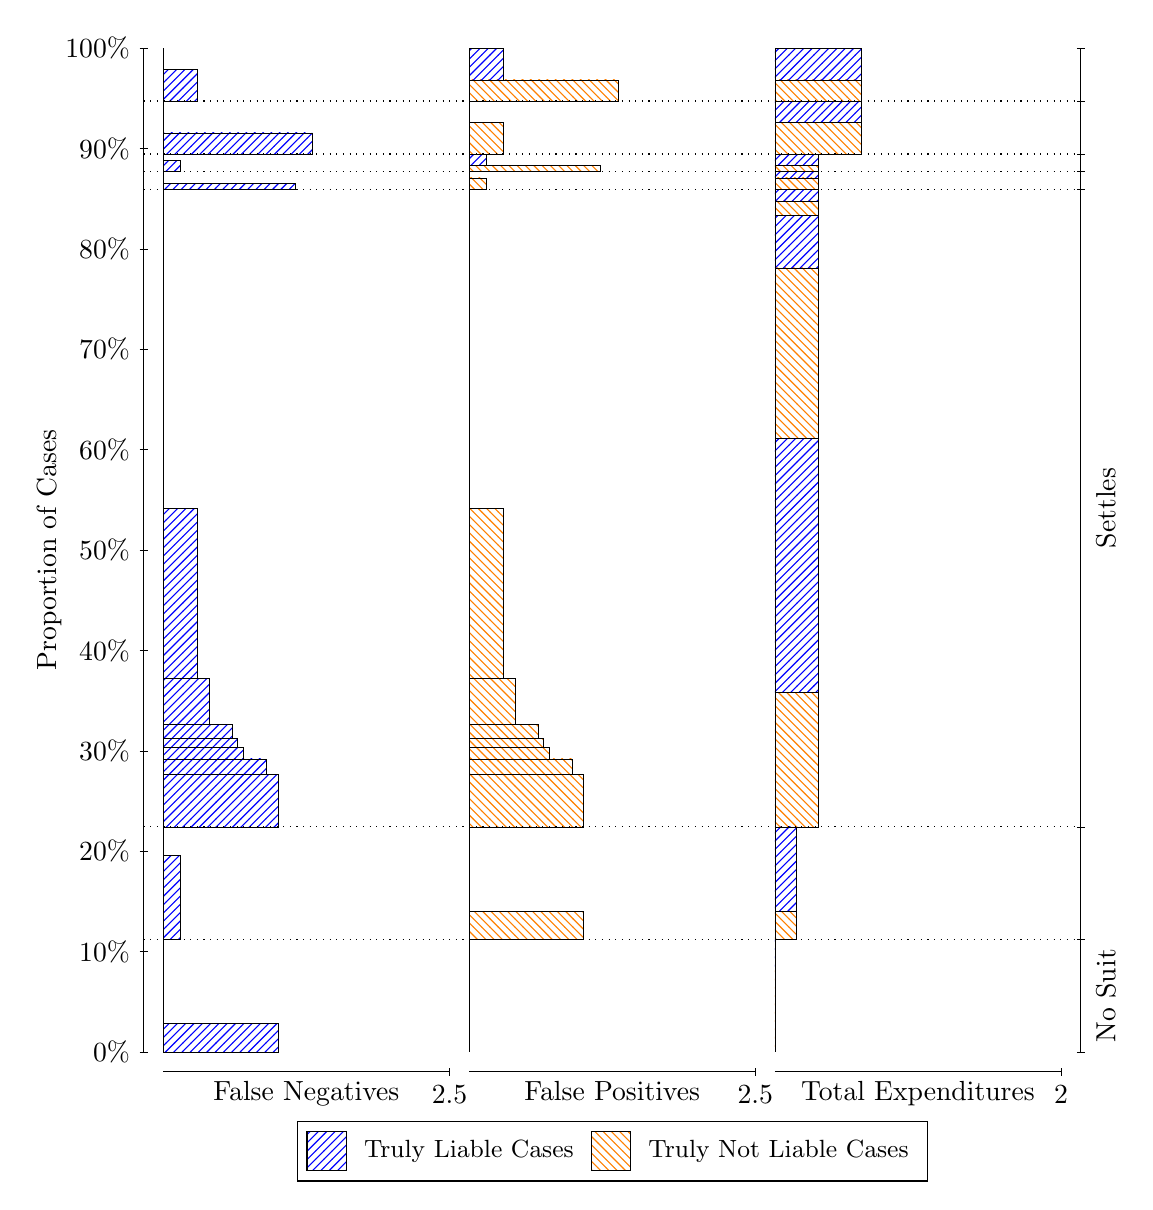
\begin{tikzpicture}
\draw[black, very thin] (1.5,1.75) -- (1.5,14.5);
\node[rotate=90, text=black, anchor=center] at (0.3, 8.125) {Proportion of Cases};
\draw[black, very thin] (1.45,1.75) -- (1.55,1.75);
\node[text=black, anchor=east] at (1.45, 1.75) {0\%};
\draw[black, very thin] (1.45,3.025) -- (1.55,3.025);
\node[text=black, anchor=east] at (1.45, 3.025) {10\%};
\draw[black, very thin] (1.45,4.3) -- (1.55,4.3);
\node[text=black, anchor=east] at (1.45, 4.3) {20\%};
\draw[black, very thin] (1.45,5.575) -- (1.55,5.575);
\node[text=black, anchor=east] at (1.45, 5.575) {30\%};
\draw[black, very thin] (1.45,6.85) -- (1.55,6.85);
\node[text=black, anchor=east] at (1.45, 6.85) {40\%};
\draw[black, very thin] (1.45,8.125) -- (1.55,8.125);
\node[text=black, anchor=east] at (1.45, 8.125) {50\%};
\draw[black, very thin] (1.45,9.4) -- (1.55,9.4);
\node[text=black, anchor=east] at (1.45, 9.4) {60\%};
\draw[black, very thin] (1.45,10.675) -- (1.55,10.675);
\node[text=black, anchor=east] at (1.45, 10.675) {70\%};
\draw[black, very thin] (1.45,11.95) -- (1.55,11.95);
\node[text=black, anchor=east] at (1.45, 11.95) {80\%};
\draw[black, very thin] (1.45,13.225) -- (1.55,13.225);
\node[text=black, anchor=east] at (1.45, 13.225) {90\%};
\draw[black, very thin] (1.45,14.5) -- (1.55,14.5);
\node[text=black, anchor=east] at (1.45, 14.5) {100\%};

\draw[black, very thin] (13.4,1.75) -- (13.4,14.5);
\draw[black, very thin] (13.35,1.75) -- (13.45,1.75);
\node[anchor=west] at (13.35, 1.75) {};
\draw[black, very thin] (13.35,3.1795) -- (13.45,3.1795);
\node[anchor=west] at (13.35, 3.1795) {};
\draw[black, very thin] (13.35,4.6089) -- (13.45,4.6089);
\node[anchor=west] at (13.35, 4.6089) {};
\draw[black, very thin] (13.35,12.706) -- (13.45,12.706);
\node[anchor=west] at (13.35, 12.706) {};
\draw[black, very thin] (13.35,12.93) -- (13.45,12.93);
\node[anchor=west] at (13.35, 12.93) {};
\draw[black, very thin] (13.35,13.154) -- (13.45,13.154);
\node[anchor=west] at (13.35, 13.154) {};
\draw[black, very thin] (13.35,13.827) -- (13.45,13.827);
\node[anchor=west] at (13.35, 13.827) {};
\draw[black, very thin] (13.35,14.5) -- (13.45,14.5);
\node[anchor=west] at (13.35, 14.5) {};

\draw[black, very thin, pattern color=blue, pattern=north east lines] (1.75,1.75) rectangle (3.2033,2.11);
\draw[black, very thin, pattern color=orange, pattern=north west lines] (1.75,2.11) rectangle (1.75,3.1795);
\draw[black, very thin, pattern color=blue, pattern=north east lines] (1.75,3.1795) rectangle (1.968,4.249);
\draw[black, very thin, pattern color=orange, pattern=north west lines] (1.75,4.249) rectangle (1.75,4.6089);
\draw[black, very thin, pattern color=blue, pattern=north east lines] (1.75,4.6089) rectangle (3.2033,5.2787);
\draw[black, very thin, pattern color=blue, pattern=north east lines] (1.75,5.2787) rectangle (3.058,5.4734);
\draw[black, very thin, pattern color=blue, pattern=north east lines] (1.75,5.4734) rectangle (2.7673,5.6204);
\draw[black, very thin, pattern color=blue, pattern=north east lines] (1.75,5.6204) rectangle (2.6947,5.7286);
\draw[black, very thin, pattern color=blue, pattern=north east lines] (1.75,5.7286) rectangle (2.622,5.9098);
\draw[black, very thin, pattern color=blue, pattern=north east lines] (1.75,5.9098) rectangle (2.3313,6.4935);
\draw[black, very thin, pattern color=blue, pattern=north east lines] (1.75,6.4935) rectangle (2.186,8.6573);
\draw[black, very thin, pattern color=orange, pattern=north west lines] (1.75,8.6573) rectangle (1.75,12.706);
\draw[black, very thin, pattern color=blue, pattern=north east lines] (1.75,12.706) rectangle (3.4213,12.784);
\draw[black, very thin, pattern color=orange, pattern=north west lines] (1.75,12.784) rectangle (1.75,12.93);
\draw[black, very thin, pattern color=blue, pattern=north east lines] (1.75,12.93) rectangle (1.968,13.076);
\draw[black, very thin, pattern color=orange, pattern=north west lines] (1.75,13.076) rectangle (1.75,13.154);
\draw[black, very thin, pattern color=blue, pattern=north east lines] (1.75,13.154) rectangle (3.6393,13.422);
\draw[black, very thin, pattern color=orange, pattern=north west lines] (1.75,13.422) rectangle (1.75,13.827);
\draw[black, very thin, pattern color=blue, pattern=north east lines] (1.75,13.827) rectangle (2.186,14.232);
\draw[black, very thin, pattern color=orange, pattern=north west lines] (1.75,14.232) rectangle (1.75,14.5);
\draw[black, very thin, pattern color=orange, pattern=north west lines] (5.6333,1.75) rectangle (5.6333,2.8195);
\draw[black, very thin, pattern color=blue, pattern=north east lines] (5.6333,2.8195) rectangle (5.6333,3.1795);
\draw[black, very thin, pattern color=orange, pattern=north west lines] (5.6333,3.1795) rectangle (7.0867,3.5394);
\draw[black, very thin, pattern color=blue, pattern=north east lines] (5.6333,3.5394) rectangle (5.6333,4.6089);
\draw[black, very thin, pattern color=orange, pattern=north west lines] (5.6333,4.6089) rectangle (7.0867,5.2787);
\draw[black, very thin, pattern color=orange, pattern=north west lines] (5.6333,5.2787) rectangle (6.9413,5.4733);
\draw[black, very thin, pattern color=orange, pattern=north west lines] (5.6333,5.4733) rectangle (6.6507,5.6204);
\draw[black, very thin, pattern color=orange, pattern=north west lines] (5.6333,5.6204) rectangle (6.578,5.7285);
\draw[black, very thin, pattern color=orange, pattern=north west lines] (5.6333,5.7285) rectangle (6.5053,5.9098);
\draw[black, very thin, pattern color=orange, pattern=north west lines] (5.6333,5.9098) rectangle (6.2147,6.4935);
\draw[black, very thin, pattern color=orange, pattern=north west lines] (5.6333,6.4935) rectangle (6.0693,8.6574);
\draw[black, very thin, pattern color=blue, pattern=north east lines] (5.6333,8.6574) rectangle (5.6333,12.706);
\draw[black, very thin, pattern color=orange, pattern=north west lines] (5.6333,12.706) rectangle (5.8513,12.852);
\draw[black, very thin, pattern color=blue, pattern=north east lines] (5.6333,12.852) rectangle (5.6333,12.93);
\draw[black, very thin, pattern color=orange, pattern=north west lines] (5.6333,12.93) rectangle (7.3047,13.008);
\draw[black, very thin, pattern color=blue, pattern=north east lines] (5.6333,13.008) rectangle (5.8513,13.154);
\draw[black, very thin, pattern color=orange, pattern=north west lines] (5.6333,13.154) rectangle (6.0693,13.559);
\draw[black, very thin, pattern color=blue, pattern=north east lines] (5.6333,13.559) rectangle (5.6333,13.827);
\draw[black, very thin, pattern color=orange, pattern=north west lines] (5.6333,13.827) rectangle (7.5227,14.095);
\draw[black, very thin, pattern color=blue, pattern=north east lines] (5.6333,14.095) rectangle (6.0693,14.5);
\draw[black, very thin, pattern color=orange, pattern=north west lines] (9.5167,1.75) rectangle (9.5167,2.8195);
\draw[black, very thin, pattern color=blue, pattern=north east lines] (9.5167,2.8195) rectangle (9.5167,3.1795);
\draw[black, very thin, pattern color=orange, pattern=north west lines] (9.5167,3.1795) rectangle (9.7892,3.5394);
\draw[black, very thin, pattern color=blue, pattern=north east lines] (9.5167,3.5394) rectangle (9.7892,4.6089);
\draw[black, very thin, pattern color=orange, pattern=north west lines] (9.5167,4.6089) rectangle (10.062,6.3122);
\draw[black, very thin, pattern color=blue, pattern=north east lines] (9.5167,6.3122) rectangle (10.062,9.5438);
\draw[black, very thin, pattern color=orange, pattern=north west lines] (9.5167,9.5438) rectangle (10.062,11.708);
\draw[black, very thin, pattern color=blue, pattern=north east lines] (9.5167,11.708) rectangle (10.062,12.377);
\draw[black, very thin, pattern color=orange, pattern=north west lines] (9.5167,12.377) rectangle (10.062,12.559);
\draw[black, very thin, pattern color=blue, pattern=north east lines] (9.5167,12.559) rectangle (10.062,12.706);
\draw[black, very thin, pattern color=orange, pattern=north west lines] (9.5167,12.706) rectangle (10.062,12.852);
\draw[black, very thin, pattern color=blue, pattern=north east lines] (9.5167,12.852) rectangle (10.062,12.93);
\draw[black, very thin, pattern color=orange, pattern=north west lines] (9.5167,12.93) rectangle (10.062,13.008);
\draw[black, very thin, pattern color=blue, pattern=north east lines] (9.5167,13.008) rectangle (10.062,13.154);
\draw[black, very thin, pattern color=orange, pattern=north west lines] (9.5167,13.154) rectangle (10.607,13.559);
\draw[black, very thin, pattern color=blue, pattern=north east lines] (9.5167,13.559) rectangle (10.607,13.827);
\draw[black, very thin, pattern color=orange, pattern=north west lines] (9.5167,13.827) rectangle (10.607,14.095);
\draw[black, very thin, pattern color=blue, pattern=north east lines] (9.5167,14.095) rectangle (10.607,14.5);
\draw[black, dotted] (1.5,3.1795) -- (13.4,3.1795);
\draw[black, dotted] (1.5,4.6089) -- (13.4,4.6089);
\draw[black, dotted] (1.5,12.706) -- (13.4,12.706);
\draw[black, dotted] (1.5,12.93) -- (13.4,12.93);
\draw[black, dotted] (1.5,13.154) -- (13.4,13.154);
\draw[black, dotted] (1.5,13.827) -- (13.4,13.827);
\draw[black, very thin] (1.75,1.5) -- (5.3833,1.5);
\node[text=black, anchor=north] at (3.5667, 1.5) {False Negatives};
\draw[black, very thin] (5.3833,1.45) -- (5.3833,1.55);
\node[text=black, anchor=north] at (5.3833, 1.45) {2.5};

\draw[black, very thin] (5.6333,1.5) -- (9.2667,1.5);
\node[text=black, anchor=north] at (7.45, 1.5) {False Positives};
\draw[black, very thin] (9.2667,1.45) -- (9.2667,1.55);
\node[text=black, anchor=north] at (9.2667, 1.45) {2.5};

\draw[black, very thin] (9.5167,1.5) -- (13.15,1.5);
\node[text=black, anchor=north] at (11.333, 1.5) {Total Expenditures};
\draw[black, very thin] (13.15,1.45) -- (13.15,1.55);
\node[text=black, anchor=north] at (13.15, 1.45) {2};

\node[text=black, centered, rotate=90] at (13.72, 2.4647) {\contour{white}{No Suit}};

\node[text=black, centered, rotate=90] at (13.72, 8.6574) {\contour{white}{Settles}};





\draw (7.449999999999999,1.5) node[draw=none] (baseCoordinate) {};
\begin{scope}[align=center]
        \matrix[scale=0.5, draw=black, below=0.5cm of baseCoordinate, nodes={draw}, column sep=0.1cm]{
            \node[rectangle, draw, minimum width=0.5cm, minimum height=0.5cm, pattern color=blue, pattern=north east lines] {}; &
            \node[draw=none, font=\small, text=black] (B) {Truly Liable Cases}; &
            \node[rectangle, draw, minimum width=0.5cm, minimum height=0.5cm, pattern color=orange, pattern=north west lines] {}; &
            \node[draw=none, font=\small, text=black] (B) {Truly Not Liable Cases}; \\
            };
\end{scope}

\end{tikzpicture}
\end{document}